\chapter{ROS OpenAI Gym}

Here we will try to implement the q learning based controller for drone in ros. Lets try to send drone from point A to B.


\section{ARdrone}
ARdrone most popular drone often used with the simulation using the ros.
\begin{figure}
    \centering
    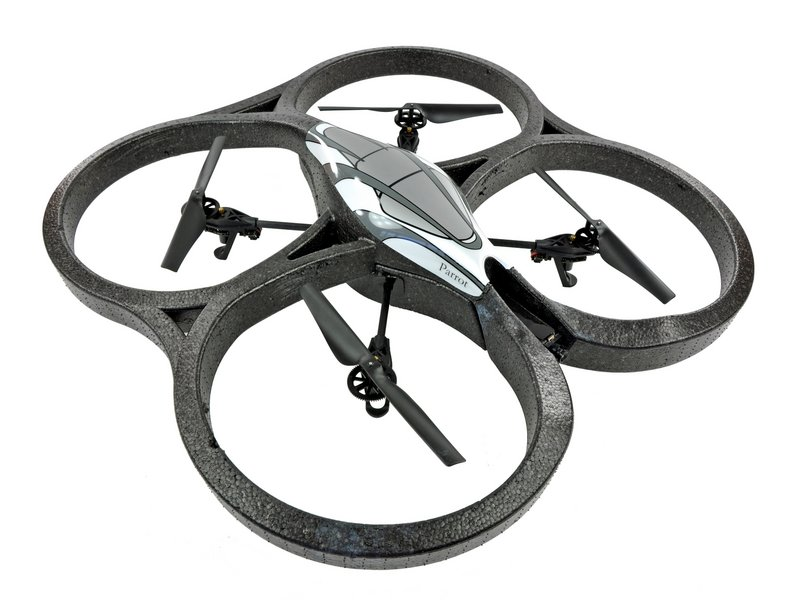
\includegraphics[width=0.5\textwidth]{images/ardrone.jpg}
    \caption{Ardrone}
\end{figure}
\section{ROS development studio}
I used the online ros development studio by \textbf{theconstruct} for simulating RL algorithm on the drone as my local system was not powerful enough to take heavy load.

\begin{figure}
    \centering
    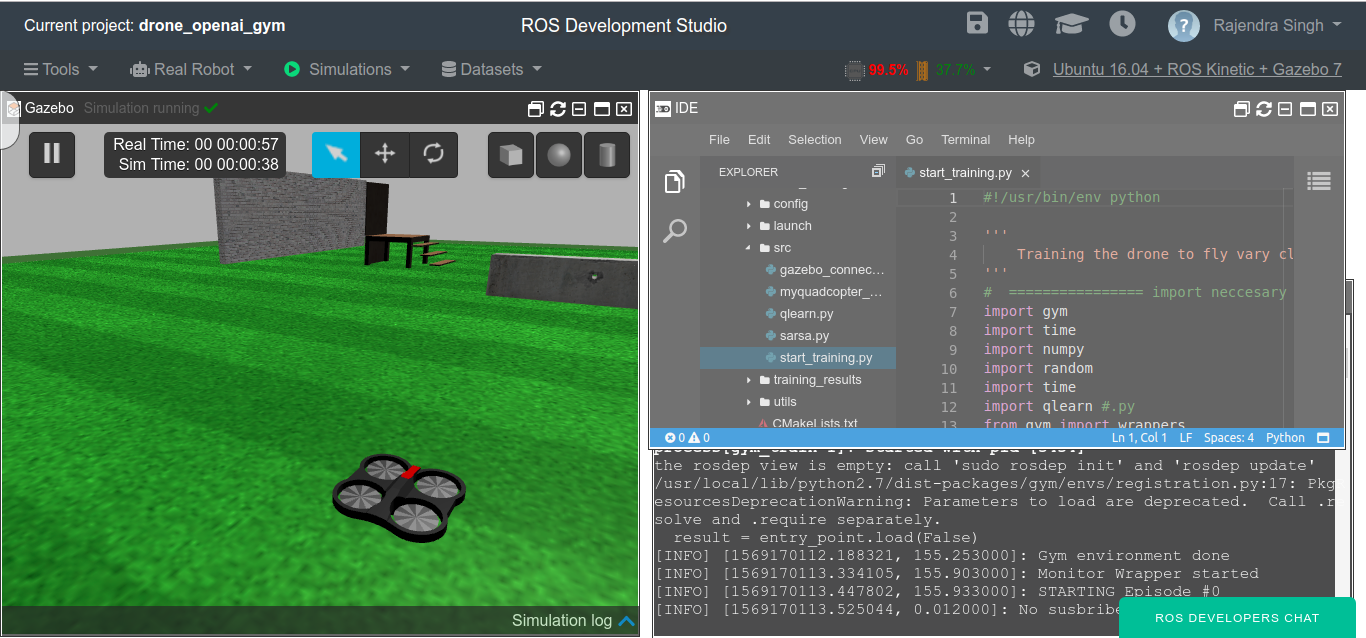
\includegraphics[width=\textwidth]{images/rds.png}
    \caption{Simulation of ARdrone on ROS Development studio}
\end{figure}
\section{Algorithm}

This code is inspired by another rosject at theconstruct, let's try to understand it. 

\textbf{Code}
\begin{minted}{python}
#!/usr/bin/env python

'''
    Training the drone to fly from point A to point B.
'''
#  ================ import neccesary for gym ============= #
import gym
import time
import numpy
import random
import time
import qlearn #.py
from gym import wrappers
# =============== required ROS libraries ================#
import rospy
import rospkg
# ========== import our training environment ============#
import myquadcopter_env #.py

if __name__ == '__main__':
    rospy.init_node('drone_gym', anonymous=True)
    # ======= Create the Gym environment ===#
    env = gym.make('QuadcopterLiveShow-v0')
    rospy.loginfo ( "Gym environment done")
    # ============== Set the logging system ==================#
    rospack = rospkg.RosPack()
    pkg_path = rospack.get_path('drone_training')
    outdir = pkg_path + '/training_results'
    env = wrappers.Monitor(env, outdir, force=True)
    rospy.loginfo ( "Monitor Wrapper started")
    last_time_steps = numpy.ndarray(0)
    # load param form yaml file
    Alpha = rospy.get_param("/alpha")
    Epsilon = rospy.get_param("/epsilon")
    Gamma = rospy.get_param("/gamma")
    epsilon_discount = rospy.get_param("/epsilon_discount")
    nepisodes = rospy.get_param("/nepisodes")
    nsteps = rospy.get_param("/nsteps")
    # Initialises(class) the algorithm that we are going to use for learning
    qlearn = qlearn.QLearn(actions=range(env.action_space.n), alpha=Alpha, gamma=Gamma, epsilon=Epsilon)
    initial_epsilon = qlearn.epsilon
    start_time = time.time()
    highest_reward = 0

    # for nepisodes
    for x in range(nepisodes):
        rospy.loginfo ("STARTING Episode #"+str(x))
        cumulated_reward = 0
        done = False
        if qlearn.epsilon > 0.05: #epsilon delay
            qlearn.epsilon *= epsilon_discount
        observation = env.reset()# Initialize the environment and get first state of the robot
        state = ''.join(map(str, observation))
        #env.render()   # Show on screen the actual situation of the robot
        # ==== while nsteps or not done ====#
        for i in range(nsteps):
            action = qlearn.chooseAction(state)# Pick an action based on the current state
            observation, reward, done, info = env.step(action)# Execute the action in the environment and get feedback
            cumulated_reward += reward
            if highest_reward < cumulated_reward:#update the highest_reward
                highest_reward = cumulated_reward
            nextState = ''.join(map(str, observation))#next state
            qlearn.learn(state, action, reward, nextState)# Make the algorithm learn based on the results
            if not(done):
                state = nextState
            else:
                rospy.loginfo ("DONE")
                last_time_steps = numpy.append(last_time_steps, [int(i + 1)])
                break
        #getting hours, minutes and secounds
        m, s = divmod(int(time.time() - start_time), 60)
        h, m = divmod(m, 60)
        rospy.loginfo ( ("EP: "+str(x+1)+" - [alpha: "+str(round(qlearn.alpha,2))+" - gamma: "+str(round(qlearn.gamma,2))+" - epsilon: "+str(round(qlearn.epsilon,2))+"] - Reward: "+str(cumulated_reward)+"     Time: %d:%02d:%02d" % (h, m, s)))
    rospy.loginfo ( ("\n|"+str(nepisodes)+"|"+str(qlearn.alpha)+"|"+str(qlearn.gamma)+"|"+str(initial_epsilon)+"*"+str(epsilon_discount)+"|"+str(highest_reward)+"| PICTURE |"))
    l = last_time_steps.tolist()
    l.sort()
    #print("Parameters: a="+str)
    rospy.loginfo("Overall score: {:0.2f}".format(last_time_steps.mean()))
    rospy.loginfo("Best 100 score: {:0.2f}".format(reduce(lambda x, y: x + y, l[-100:]) / len(l[-100:])))
    env.close() #close env

\end{minted}
% \newcommand{}[]{}
\textbf{Note:}\\
1.) In above code we import the myquadcopter-env.py, this is a openai gym environment made using ARdrone gazebo simulation and It is not written by me.
\section{Conclusion}
In this chapter, we proposed another algorithm to control the drone, which is based on the Q learning. As this task not just required the good understanding of Q learning but also required very good understanding of ROS and gazebo, ARdrone simulation and ros message and topics.
Hence, It was not possible for me to write whole code myself and therefore I used libraries for some part, e.g. myquadcopter-env.py as mentioned above. In future, I'll learn and try to write the env also myself.

